\let\negmedspace\undefined
\let\negthickspace\undefined
\documentclass[12pt]{article}
\usepackage{cite}
\usepackage{float}
\usepackage{amsmath,amssymb,amsfonts,amsthm}
\usepackage{algorithmic}
\usepackage{graphicx}
\usepackage{textcomp}
\usepackage{xcolor}
\usepackage{txfonts}
\usepackage{listings}
\usepackage{enumitem}
\usepackage{mathtools}
\usepackage{gensymb}
\usepackage{comment}
\usepackage[breaklinks=true]{hyperref}
\usepackage{tkz-euclide} 
\usepackage{listings}
\usepackage{gvv}                                                             
\usepackage{gvv-book}     
\usepackage{xparse}
\usepackage{color}                                            
\usepackage{array}                                            
\usepackage{longtable}                                       
\usepackage{calc}                                             
\usepackage{multirow}
\usepackage{multicol}
\usepackage{hhline}                                           
\usepackage{ifthen}                                           
\usepackage{lscape}
\usepackage{tabularx}
\usepackage{array}
\usepackage{float}
\usepackage{geometry}
\geometry{left=1in, right=1in, top=1in, bottom=1in}

\begin{document}

\begin{center}
    {\LARGE \textbf{EC : ELECTRONICS AND COMMUNICATION ENGINEERING}}\\[0.7em]
    \textbf{Duration:} Three Hours
    \hspace{2cm}
    \textbf{Maximum Marks:} 150
\end{center}


\textbf{Read the following instructions carefully}
\begin{enumerate}[leftmargin=2em,itemsep=0.5em]
    \item This question paper contains \textbf{28 printed pages} including pages for rough work. Please check all pages and report discrepancy, if any.
    \item Write your registration number, your name and name of the examination centre at the specified locations on the right half of the ORS.
    \item Using \textbf{HB pencil}, darken the appropriate bubble under each digit of your registration number and the letters corresponding to your paper code.
    \item All the questions in this question paper are of \textbf{objective type}.
    \item Questions must be answered on Objective Response Sheet (\textbf{ORS}) by darkening the appropriate bubble (marked A, B, C, D) using HB pencil against the question number on the left hand side of the ORS. \textbf{Each question has only one correct answer.} In case you wish to change an answer, erase the old answer completely. More than one answer bubbled against a question will be treated as a wrong answer.
    \item Questions 1 through 20 are 1-mark questions and questions 21 through 85 are 2-mark questions.
    \item Questions 71 through 73 is one set of common data questions, questions 74 and 75 is another pair of common data questions. The question pairs (76, 77), (78, 79), (80, 81), (82, 83) and (84, 85) are questions with linked answers. The answer to the second question of the above pairs will depend on the answer to the first question of the pair. If the first question in the linked pair is wrongly answered or is un-attempted, then the answer to the second question in the pair will not be evaluated.
    \item Un-attempted questions will carry zero marks.
     \large \textbf {NEGATIVE MARKING:} For Q.1 to Q.20, \textbf{0.25 mark will be deducted for each wrong answer}. For Q.21 to Q.75, \textbf{0.5 mark will be deducted for each wrong answer}. For the pairs of questions with linked answers, there will be negative marks only for wrong answer to the first question, i.e. for Q.76, Q.78, Q.80, Q.82 and Q.84, \textbf{0.5 mark will be deducted for each wrong answer}. There is no negative marking for Q.77, Q.79, Q.81, Q.83 and Q.85.
    \item Calculator \textbf{without data connectivity} is allowed in the examination hall.
    \item Charts, graph sheets and tables are NOT allowed in the examination hall.
    \item Rough work can be done on the question paper itself. Additional blank pages are given at the end of the question paper for rough work.
\end{enumerate}



\newpage

\section*{Q.1 -- Q.20 carry one mark each.}

\begin{enumerate}[leftmargin=2.5em, label=\textbf{Q.\arabic*}., itemsep=2em]
\item All the four entries of the $2\times2$ matrix $\mathbf{P} = \myvec{P_{11} & P_{12}\\ P_{21} & P_{22}}$ are nonzero, and one of its eigenvalues is zero. Which of the following statements is true?
 
\noindent \textbf{[GATE EE 2025]}
\begin{multicols}{2}
    \begin{enumerate}
        \item $P_{11}P_{22} - P_{12}P_{21} = 1$
        \item $P_{11}P_{22} - P_{12}P_{21} = -1$
        \item $P_{11}P_{22} - P_{12}P_{21} = 0$
        \item $P_{11}P_{22} + P_{12}P_{21} = 0$
    \end{enumerate}
\end{multicols}

\item The system of linear equations
\begin{align}
4x + 2y &= 7 \\
2x + y  &= 6
\end{align}
has
 
\noindent \textbf{[GATE EE 2025]}
\begin{multicols}{2}
    \begin{enumerate}
        \item a unique solution
        \item no solution
        \item an infinite number of solutions
        \item exactly two distinct solutions
    \end{enumerate}
\end{multicols}

\item The equation $\sin(z) = 10$ has
 
\noindent \textbf{[GATE EE 2025]}
    \begin{enumerate}
        \item no real or complex solution
        \item exactly two dinumber of trees (P) and the number of cut-sets (Q) are
stinct complex solutions
        \item a unique solution
        \item an infinite number of complex solutions
    \end{enumerate}

\item For real values of $x$, the minimum value of the function $f(x) = \exp(x) + \exp(-x)$ is
 
\noindent \textbf{[GATE EE 2025]}
\begin{multicols}{4}
    \begin{enumerate}
        \item 2
        \item 1
        \item 0.5
        \item 0
    \end{enumerate}
\end{multicols}

\item Which of the following functions would have only odd powers of $x$ in its Taylor series expansion about the point $x = 0$?
 
\noindent \textbf{[GATE EE 2025]}
\begin{multicols}{4}
    \begin{enumerate}
        \item $\sin(x^3)$
        \item $\sin(x^2)$
        \item $\cos(x^3)$
        \item $\cos(x^2)$
    \end{enumerate}
\end{multicols}

\item Which of the following is a solution to the differential equation $\dfrac{dx(t)}{dt} + 3x(t) = 0$?
 
\noindent \textbf{[GATE EE 2025]}
\begin{multicols}{4}
    \begin{enumerate}
        \item $x(t) = 3e^{-t}$
        \item $x(t) = 2e^{-3t}$
        \item $x(t) = \dfrac{3}{2} t^2$
        \item $x(t) = 3t^2$
    \end{enumerate}
\end{multicols}

\item In the following graph, the number of trees (P) and the number of cut-sets (Q) are
number of trees (P) and the number of cut-sets (Q) are
\noindent \textbf{[GATE EE 2025]}
\begin{figure}[H]\centering
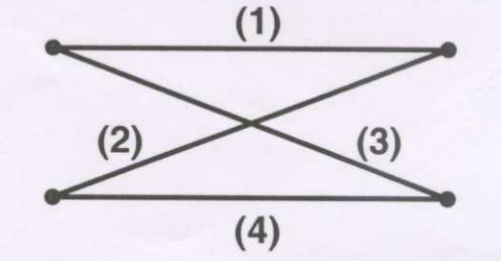
\includegraphics[width=0.5\columnwidth]{figs/q7.png}
\caption{Diagram}
\label{fig:q7}
\end{figure}
\begin{multicols}{4}
    \begin{enumerate}
        \item P=2, Q=2
        \item P=2, Q=6
        \item P=4, Q=6
        \item P=4, Q=10
    \end{enumerate}
\end{multicols}

\item In the following circuit, the switch $S$ is closed at $t = 0$. The rate of change of current $\dfrac{di}{dt}(0^+)$ is given by
 
\noindent \textbf{[GATE EE 2025]}
\begin{figure}[H]\centering
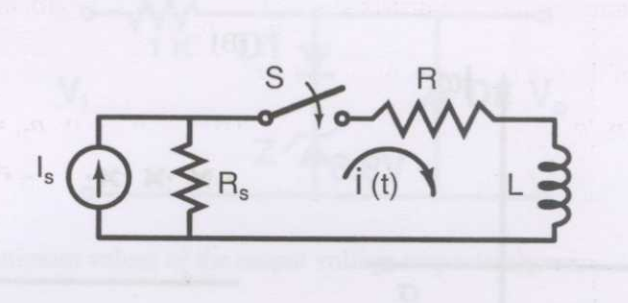
\includegraphics[width=0.5\columnwidth]{figs/q8.png}
\caption{Circuit}
\label{fig:q8}
\end{figure}
\begin{multicols}{4}
\begin{enumerate}
    \item 0
    \item $\dfrac{R_s I_s}{L}$
    \item $\dfrac{(R+R_s) I_s}{L}$
    \item $\infty$
\end{enumerate}
\end{multicols}

\item The input and output of a continuous time system are respectively denoted by $x(t)$ and $y(t)$. Which of the following descriptions corresponds to a causal system?
 
\noindent \textbf{[GATE EE 2025]}
\begin{multicols}{2}
\begin{enumerate}
    \item $y(t) = x(t-2) + x(t+4)$
    \item $y(t) = (t-4) x(t+1)$
    \item $y(t) = (t+4) x(t-1)$
    \item $y(t) = (t+5) x(t+5)$
\end{enumerate}
\end{multicols}

\item The impulse response $h(t)$ of a linear time-invariant continuous time system is described by $h(t) = \exp(\alpha t) u(t) + \exp(\beta t) u(t)$, where $u(t)$ denotes the unit step function, and $\alpha$ and $\beta$ are real constants. This system is stable if
 
\noindent \textbf{[GATE EE 2025]}
\begin{multicols}{2}
\begin{enumerate}
    \item $\alpha$ is positive and $\beta$ is positive
    \item $\alpha$ is negative and $\beta$ is negative
    \item $\alpha$ is positive and $\beta$ is negative
    \item $\alpha$ is negative and $\beta$ is positive
\end{enumerate}
\end{multicols}

\item The pole-zero plot given below corresponds to a
 
\noindent \textbf{[GATE EE 2025]}
\begin{figure}[H]\centering
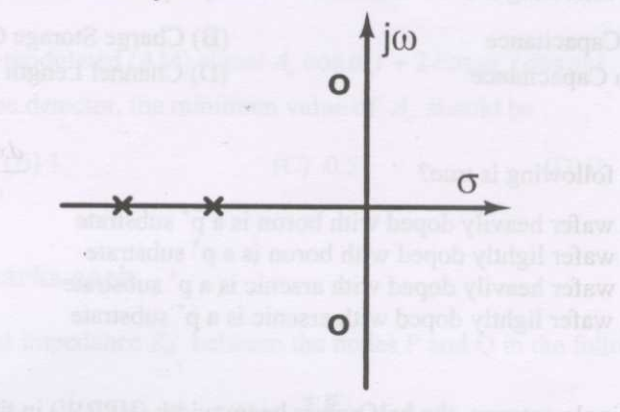
\includegraphics[width=0.5\columnwidth]{figs/q11.png}
\caption{Graph}
\label{fig:q11}
\end{figure}
\begin{multicols}{2}
\begin{enumerate}
    \item Low pass filter
    \item High pass filter
    \item Band pass filter
    \item Notch filter
\end{enumerate}
\end{multicols}
\item Step responses of a set of three second-order underdamped systems all have the same percentage overshoot. Which of the following diagrams represents the poles of the three systems?\\
 
\noindent \textbf{[GATE EE 2025]}
\begin{figure}[H]\centering
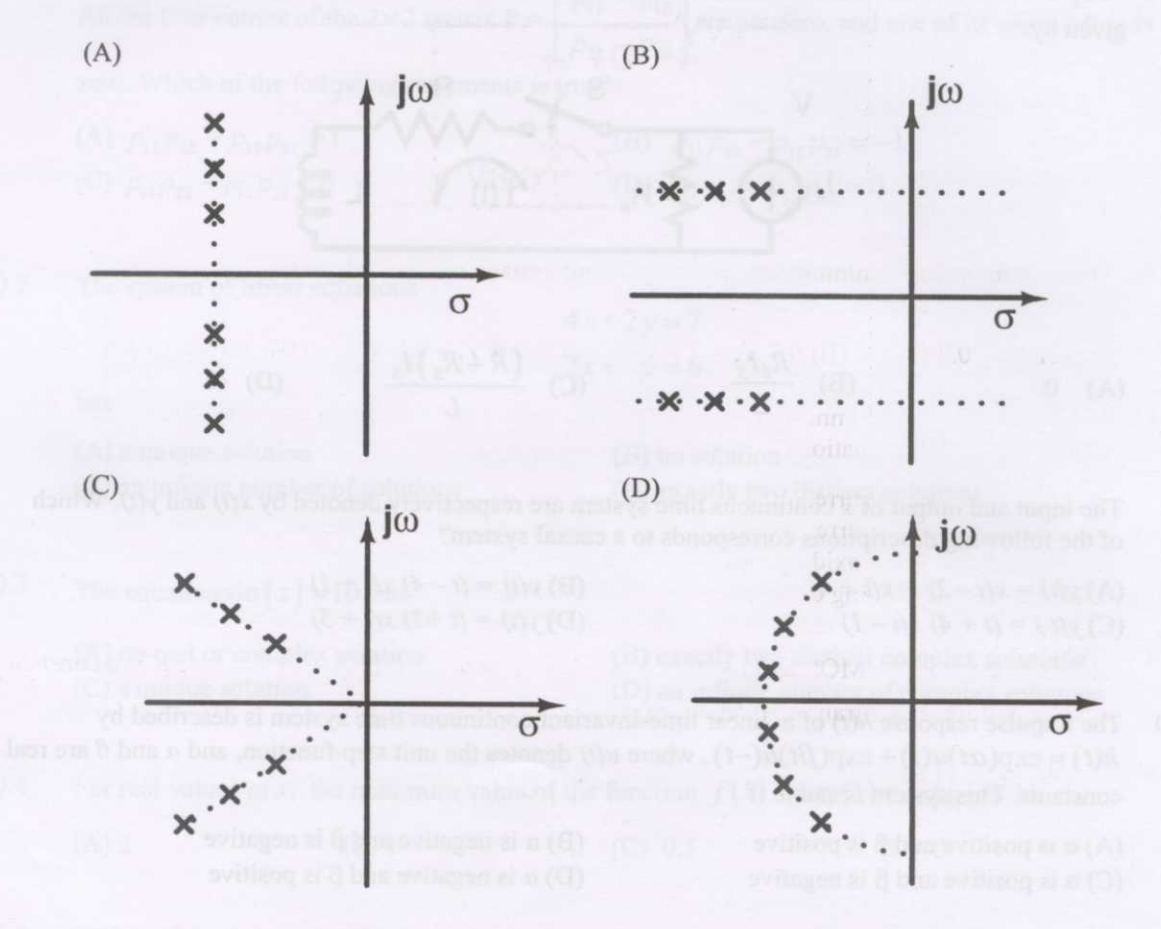
\includegraphics[width=0.95\columnwidth]{figs/q12.png}
\caption{Options}
\label{fig:q12}
\end{figure}
\begin{multicols}{4}
\begin{enumerate}
  \item (A)
  \item (B)
  \item (C)
  \item (D)
\end{enumerate}
\end{multicols}

\item
Which of the following is NOT associated with a p-n junction?
 
\noindent \textbf{[GATE EE 2025]}
\begin{multicols}{2}
\begin{enumerate}
  \item Junction Capacitance
  \item Charge Storage Capacitance
  \item Depletion Capacitance
  \item Channel Length Modulation
\end{enumerate}
\end{multicols}

\item
Which of the following is true?
 
\noindent \textbf{[GATE EE 2025]}
\begin{enumerate}
  \item A silicon wafer heavily doped with boron is a p$^+$ substrate
  \item A silicon wafer lightly doped with boron is a p$^+$ substrate
  \item A silicon wafer heavily doped with arsenic is a p$^+$ substrate
  \item A silicon wafer lightly doped with arsenic is a p$^+$ substrate
\end{enumerate}

\item
For a Hertz dipole antenna, the half power beam width (HPBW) in the E-plane is
 
\noindent \textbf{[GATE EE 2025]}
\begin{multicols}{4}
\begin{enumerate}
  \item 360\degree
  \item 180\degree
  \item 90\degree
  \item 45\degree
\end{enumerate}
\end{multicols}

\item
For static electric and magnetic fields in an inhomogeneous source-free medium, which of the following represents the correct form of two of Maxwell's equations?

\noindent \textbf{[GATE EE 2025]}
\begin{multicols}{2}
\begin{enumerate}
  \item $\nabla \cdot E = 0$, \quad $\nabla \times B = 0$
  \item $\nabla \cdot E = 0$, \quad $\nabla \cdot B = 0$
  \item $\nabla \times E = 0$, \quad $\nabla \times B = 0$
  \item $\nabla \times E = 0$, \quad $\nabla \cdot B = 0$
\end{enumerate}
\end{multicols}


\item In the following limiter circuit, an input voltage $V_i=10\sin100\pi t$ is applied. Assume the diode drop is $0.7$ V when forward biased. The Zener breakdown voltage is $6.8$ V.
\begin{figure}[H]\centering
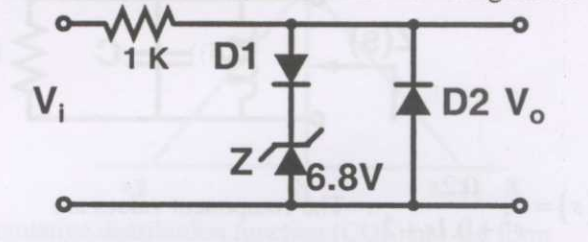
\includegraphics[width=0.7\columnwidth]{figs/q17.png}
\caption{Circuit}
\label{fig:q17}
\end{figure}

The maximum and minimum values of the output voltage respectively are
 
\noindent \textbf{[GATE EE 2025]}
\begin{multicols}{4}
\begin{enumerate}
  \item $6.1$ V, $-0.7$ V
  \item $0.7$ V, $-7.5$ V
  \item $7.5$ V, $-0.7$ V
  \item $7.5$ V, $-7.5$ V
\end{enumerate}
\end{multicols}

\item A silicon wafer has $100\,\mathrm{nm}$ of oxide on it and is inserted in a furnace at a temperature above 1000\degree C for further oxidation in dry oxygen. The oxidation rate
 
\noindent \textbf{[GATE EE 2025]}
\begin{enumerate}
  \item is independent of current oxide thickness and temperature
  \item is independent of current oxide thickness but depends on temperature
  \item slows down as the oxide grows
  \item is zero as the existing oxide prevents further oxidation
\end{enumerate}

\item The drain current of a MOSFET in saturation is given by $I_D=K(V_{\mathrm{GS}}-V_T)^2$ where $K$ is a constant.
The magnitude of the transconductance $g_m$ is
 
\noindent \textbf{[GATE EE 2025]}
\begin{multicols}{4}
\begin{enumerate}
  \item $\dfrac{K(V_{\mathrm{GS}}-V_T)^2}{V_{\mathrm{DS}}}$
  \item $2K(V_{\mathrm{GS}}-V_T)$
  \item $\dfrac{I_D}{V_{\mathrm{GS}}-V_{\mathrm{DS}}}$
  \item $\dfrac{K(V_{\mathrm{GS}}-V_T)^2}{V_{\mathrm{GS}}}$
\end{enumerate}
\end{multicols}

\item Consider the amplitude modulated (AM) signal $A\cos\ohm_1 t+2\cos\ohm_2 t\cos\ohm_1 t$. For demodulating the signal using envelope detector, the minimum value of $A$ should be
 
\noindent \textbf{[GATE EE 2025]}
\begin{multicols}{4}
\begin{enumerate}
  \item 2
  \item 1
  \item 0.5
  \item 0
\end{enumerate}
\end{multicols}

\end{enumerate}


\large \textbf {Q.21 – Q.75 carry two marks each.}


\begin{enumerate}[leftmargin=*, label=\textbf{Q.\arabic*:}]
\setcounter{enumi}{20}

\item The Thevenin equivalent impedance $Z_{th}$ between the nodes $P$ and $Q$ in the following circuit is
 
\noindent \textbf{[GATE EE 2025]}
\begin{figure}[H]\centering
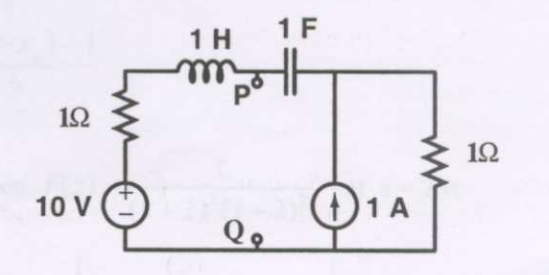
\includegraphics[width=0.7\columnwidth]{figs/q21.png}
\caption{Circuit}
\label{fig:q21}
\end{figure}
\begin{multicols}{4}
\begin{enumerate}
  \item 1
  \item $1+s+\dfrac{1}{s}$
  \item $2+s+\dfrac{1}{s}$
  \item $\dfrac{s^2+s+1}{s^2+2s+1}$
\end{enumerate}
\end{multicols}

\item The driving point impedance of the following network is given by $Z(s)=\frac{0.2s}{s^2+0.1s+2}$. The component values are
 
\noindent \textbf{[GATE EE 2025]}
\begin{figure}[H]\centering
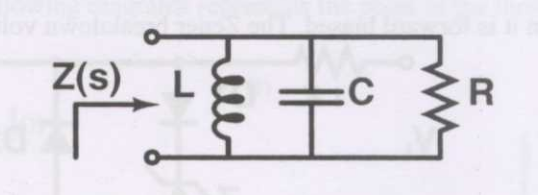
\includegraphics[width=0.7\columnwidth]{figs/q22.png}
\caption{Circuit}
\label{fig:q22}
\end{figure}

\begin{multicols}{2}
\begin{enumerate}
  \item $L=5\,\text{H}$, $R=0.5\,\ohm$, $C=0.1\,\text{F}$
  \item $L=0.1\,\text{H}$, $R=0.5\,\ohm$, $C=5\,\text{F}$
  \item $L=5\,\text{H}$, $R=2\,\ohm$, $C=0.1\,\text{F}$
  \item $L=0.1\,\text{H}$, $R=2\,\ohm$, $C=5\,\text{F}$
\end{enumerate}
\end{multicols}

\item The circuit shown in the figure is used to charge the capacitor $C$ alternately from two current sources as indicated. The switches $S_1$ and $S_2$ are mechanically coupled and connected as follows:

\textit{For $2nT \leq t < (2n+1)T,\ (n=0,1,2,\ldots)$,\ $S_1$ to $P_1$ and $S_2$ to $P_2$.}\\
\textit{For $(2n+1)T \leq t < (2n+2)T,\ (n=0,1,2,\ldots)$,\ $S_1$ to $Q_1$ and $S_2$ to $Q_2$.}
\begin{figure}[H]\centering
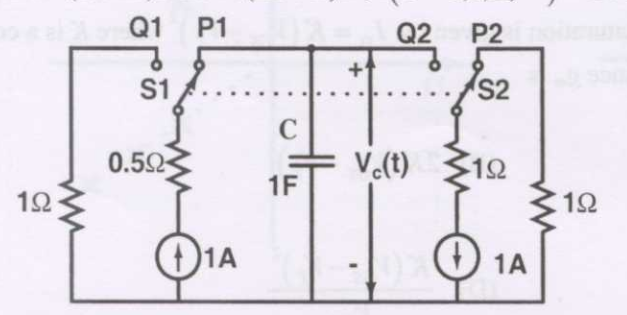
\includegraphics[width=0.7\columnwidth]{figs/q23.png}
\caption{Circuit}
\label{fig:q23}
\end{figure}
Assume that the capacitor has zero initial charge. Given that $u(t)$ is a unit step function, the voltage $V_c(t)$ across the capacitor is given by
 
\noindent \textbf{[GATE EE 2025]}
\begin{multicols}{2}
\begin{enumerate}
  \item $\displaystyle\sum_{n=0}^\infty (-1)^n t u(t-nT)$
  \item $\displaystyle u(t) + 2 \sum_{n=1}^\infty (-1)^n u(t-nT)$
  \item $\displaystyle t u(t) + 2 \sum_{n=1}^\infty (-1)^n (t-nT)u(t-nT)$
  \item $\displaystyle \sum_{n=0}^\infty \left[ 0.5 - e^{-(t-2nT)} + 0.5e^{-(t-2nT-T)} \right]$
\end{enumerate}
\end{multicols}

\newpage

\item
The probability density function (PDF) of a random variable $X$ is as shown below.

\begin{figure}[H]\centering
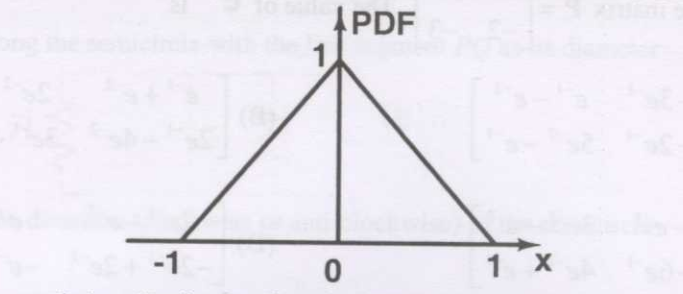
\includegraphics[width=0.5\columnwidth]{figs/q24a.png}
\caption{Graph}
\label{fig:q24a}
\end{figure}

The corresponding cumulative distribution function (CDF) has the form
 
\noindent \textbf{[GATE EE 2025]}

\begin{figure}[H]\centering
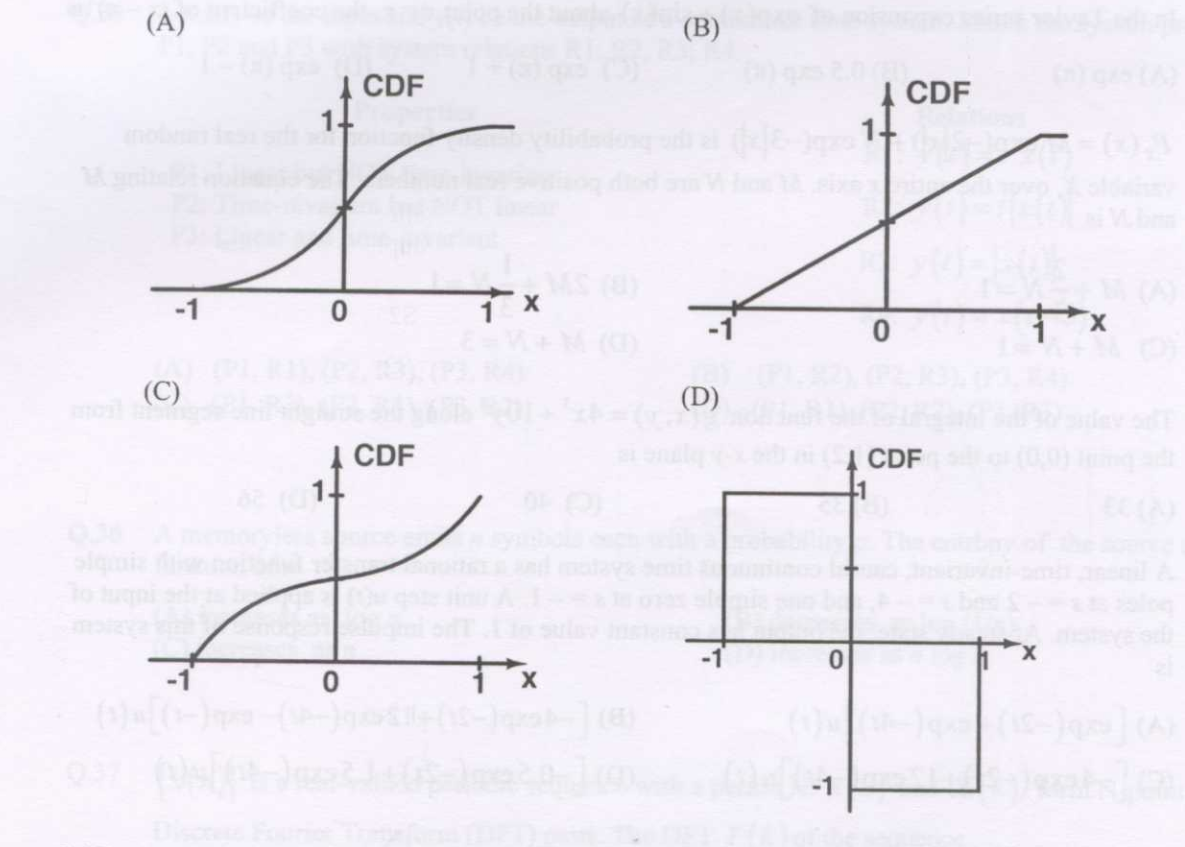
\includegraphics[width=0.95\columnwidth]{figs/q24b.png}
\caption{Options}
\label{fig:q24b}
\end{figure}

\item The recursion relation to solve $x = e^{x}$ using Newton-Raphson method is
 
\noindent \textbf{[GATE EE 2025]}
\begin{enumerate}
    \item $x_{n+1} = e^{-x_n}$
    \item $x_{n+1} = x_n - e^{-x_n}$
    \item $x_{n+1} = (1 + x_n)\dfrac{e^{-x_n}}{1 + e^{-x_n}}$
    \item $x_{n+1} = \dfrac{x_n^2 e^{-x_n} (1 + x_n) - 1}{x_n - e^{-x_n}}$
\end{enumerate}

\item The residue of the function $f(z) = \dfrac{1}{(z+2)^2 (z-2)^2}$ at $z = 2$ is
 
\noindent \textbf{[GATE EE 2025]}
\begin{multicols}{4}
\begin{enumerate}
    \item $\dfrac{1}{32}$
    \item $\dfrac{1}{16}$
    \item $\dfrac{1}{16}$
    \item $\dfrac{1}{32}$
\end{enumerate}
\end{multicols}

\item Consider the matrix $\mathbf{P} = \myvec { 0 & 1 \\ -2 & -3 }$. The value of $e^{\mathbf{P}}$ is
 
\noindent \textbf{[GATE EE 2025]}
\begin{multicols}{2}
\begin{enumerate}
    \item $\myvec { 2e^{-2} - 3e^{-1} & e^{-1} - e^{-2} \\ 2e^{-2} - 2e^{-1} & 5e^{-2} - e^{-1}}$
    \item $\myvec { e^{-1} + e^{-2} & 2e^{-2} - e^{-1} \\ 2e^{-1} - 4e^{-2} & 3e^{-1} + e^{-2} }$
    \item $\myvec { 5e^{-2} - 6e^{-1} & 3e^{-1} - e^{-2} \\ 2e^{-2} - 6e^{-1} & 4e^{-2} + e^{-1} }$
    \item $\myvec { 2e^{-1} - e^{-2} & -e^{-1} + 2e^{-2} \\ -2e^{-1} + 2e^{-2} & -e^{-1} + 2e^{-2} }$
\end{enumerate}
\end{multicols}

\item In the Taylor series expansion of $\exp(x) + \sin(x)$ about the point $x = \pi$, the coefficient of $(x - \pi)^2$ is
 
\noindent \textbf{[GATE EE 2025]}
\begin{multicols}{4}
\begin{enumerate}
    \item $\exp(\pi)$
    \item $0.5 \exp(\pi)$
    \item $\exp(\pi) + 1$
    \item $\exp(\pi) - 1$
\end{enumerate}
\end{multicols}

\item $P_X(x) = M\exp(-2|x|) + N\exp(-3|x|)$ is the probability density function for the real random variable $X$, over the entire $x$ axis. $M$ and $N$ are both positive real numbers. The equation relating $M$ and $N$ is
 
\noindent \textbf{[GATE EE 2025]}
\begin{multicols}{4}
\begin{enumerate}
    \item $M + \dfrac{2}{3} N = 1$
    \item $2M + \dfrac{1}{3}N = 1$
    \item $M + N = 1$
    \item $M + N = 3$
\end{enumerate}
\end{multicols}

\item The value of the integral of the function $g(x, y) = 4x^3 + 10y$ along the straight line segment from the point $(0,0)$ to the point $(1,2)$ in the $x-y$ plane is
 
\noindent \textbf{[GATE EE 2025]}
\begin{multicols}{4}
\begin{enumerate}
    \item $33$
    \item $35$
    \item $40$
    \item $56$
\end{enumerate}
\end{multicols}

\item A linear, time-invariant, causal continuous time system has a rational transfer function with simple poles at $s=-2$ and $s= -4$, and one simple zero at $s=-1$. A unit step $u(t)$ is applied at the input of the system. At steady state, the output has constant value of $1$. The impulse response of this system is
 
\noindent \textbf{[GATE EE 2025]}
\begin{enumerate}
    \item $\left[\exp(-2t)+\exp(-4t) \right]u(t)$
    \item $\left[ -4\exp(-2t) + 12\exp(-4t) -\exp(-t) \right]u(t)$
    \item $\left[ -4\exp(-2t) + 12\exp(-4t) \right]u(t)$
    \item $\left[ -0.5\exp(-2t) + 1.5\exp(-4t) \right]u(t)$
\end{enumerate}

\item The signal $x(t)$ is described by
\[
x(t) = \begin{cases}
1 & \text{for } -1 \leq t \leq +1 \\
0 & \text{otherwise}
\end{cases}
\]
Two of the angular frequencies at which its Fourier transform becomes zero are
 
\noindent \textbf{[GATE EE 2025]}
\begin{multicols}{4}
\begin{enumerate}
    \item $\pi,\,2\pi$
    \item $0.5\pi,\,1.5\pi$
    \item $0,\,\pi$
    \item $2\pi,\,2.5\pi$
\end{enumerate}
\end{multicols}

\item A discrete time linear shift-invariant system has an impulse response $h[n]$ with $h[0]=1$, $h[1]=-1$, $h[2]=2$, and zero otherwise. The system is given an input sequence $x[n]$ with $x[0]=x[2]=1$, and zero otherwise. The number of nonzero samples in the output sequence $y[n]$, and the value of $y[2]$ are, respectively
 
\noindent \textbf{[GATE EE 2025]}

\begin{multicols}{4}
\begin{enumerate}
    \item $5, 2$
    \item $6, 2$
    \item $6, 1$
    \item $5, 3$
\end{enumerate}
\end{multicols}

\item Consider points $P$ and $Q$ in the $x$-$y$ plane, with $P = (1,0)$ and $Q = (0,1)$. The line integral
\[
2\int_P^Q (x\,dx + y\,dy)
\]
along the semicircle with the line segment $PQ$ as its diameter
 
\noindent \textbf{[GATE EE 2025]}
\begin{enumerate}
  \item is $-1$
  \item is $0$
  \item is $1$
  \item depends on the direction (clockwise or anti-clockwise) of the semicircle
\end{enumerate}

\item Let $x(t)$ be the input and $y(t)$ be the output of a continuous time system. Match the system properties P1, P2, and P3 with system relations R1, R2, R3, R4.
\begin{figure}[H]\centering
  \begin{tabular}{ll}
    Properties & Relations \\
    P1: Linear but NOT time-invariant              & R1: $y(t)=t^2 x(t) $ \\
    P2: Time-invariant but NOT linear              & R2: $y(t)=|x(t)| $ \\
    P3: Linear and time-invariant                  & R3: $y(t)=x(t)$ \\
                                                  & R4: $y(t)=x(t-5)$
  \end{tabular}
\caption{Graph}
\label{fig:q11}
\end{figure}
 
\noindent \textbf{[GATE EE 2025]}
\begin{multicols}{2}
\begin{enumerate}
  \item (P1, R1), (P2, R3), (P3, R4)
  \item (P1, R2), (P2, R3), (P3, R4)
  \item (P1, R3), (P2, R1), (P3, R2)
  \item (P1, R1), (P2, R2), (P3, R3)
\end{enumerate}
\end{multicols}

\item A memoryless source emits $n$ symbols each with a probability $p$. The entropy of the source as a function of $n$
 
\noindent \textbf{[GATE EE 2025]}
\begin{multicols}{2}
\begin{enumerate}
  \item increases as $\log n$
  \item decreases as $\log(1/n)$
  \item increases as $n$
  \item increases as $n \log n$
\end{enumerate}
\end{multicols}

\item $\{x(n)\}$ is a real-valued periodic sequence with a period $N$. $x(n)$ and $X(k)$ form $N$-point Discrete Fourier Transform (DFT) pairs. The DFT $Y(k)$ of the sequence
\[
y(n) = x(r) x(n + r)
\]
is
 
\noindent \textbf{[GATE EE 2025]}
\begin{multicols}{2}
\begin{enumerate}
  \item $|X(k)|^2 $
  \item $\dfrac{1}{N} \sum_{r=0}^{N-1} X(r) X^*(k+r) $
  \item $\dfrac{1}{N} \sum_{r=0}^{N-1} X(r) X(k+r) $
  \item $0$
\end{enumerate}
\end{multicols}

\item
Group I lists a set of four transfer functions. Group II gives a list of possible step responses $y(t)$. Match the step responses with the corresponding transfer functions.

\textbf{Group I}

\begin{tabular}{llll}
  $P = \dfrac{25}{s^2 + 25 }$ &
  $Q = \dfrac{36}{s^2 + 20s + 36}$ &
  $R = \dfrac{36}{s^2 + 12s + 36 }$ &
  $S = \dfrac{49}{s^2 + 7s + 49}$
\end{tabular}

\textbf{Group II}
\begin{figure}[H]\centering
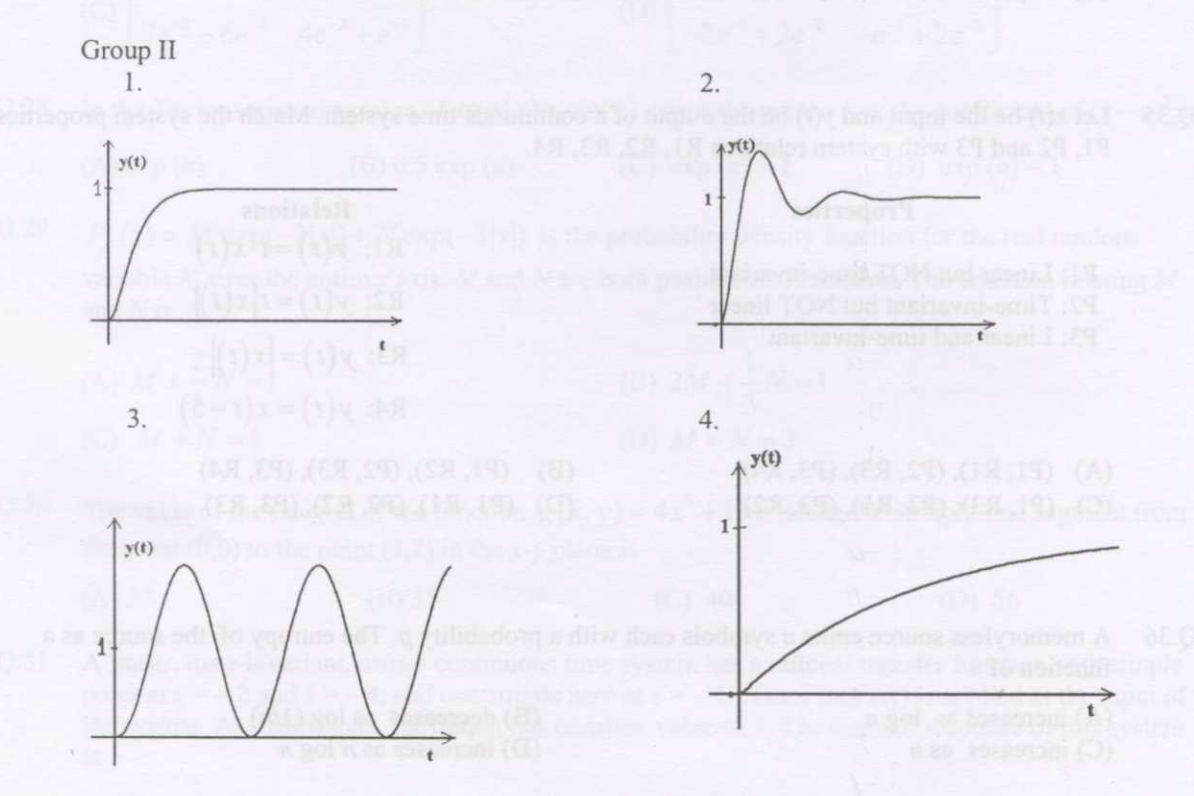
\includegraphics[width=0.9\columnwidth]{figs/q38.png}
\caption{Options}
\label{fig:q38}
\end{figure}
 
\noindent \textbf{[GATE EE 2025]}
\begin{multicols}{2}
\begin{enumerate}
  \item P-3, Q-1, R-4, S-2
  \item P-3, Q-2, R-4, S-1
  \item P-2, Q-1, R-4, S-3
  \item P-3, Q-4, R-1, S-2
\end{enumerate}
\end{multicols}

\item A certain system has transfer function $G(s) = \dfrac{s+8}{s^2 + a s - 4},$ where $a$ is a parameter. Consider the standard negative unity feedback configuration.

\begin{figure}[H]\centering
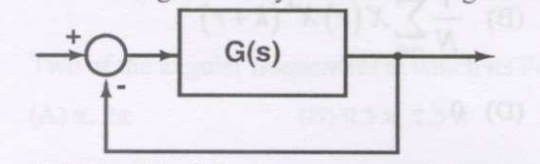
\includegraphics[width=0.5\columnwidth]{figs/q39.png}
\caption{Circuit}
\label{fig:q39}
\end{figure}

Which of the following statements is true?
 
\noindent \textbf{[GATE EE 2025]}
\begin{enumerate}
  \item The closed loop system is never stable for any value of $a$.
  \item For some positive values of $a$, the closed loop system is stable, but not for all positive values.
  \item For all positive values of $a$, the closed loop system is stable.
  \item The closed loop system is stable for all values of $a$, both positive and negative.
\end{enumerate}
\newpage
\item A signal flow graph of a system is given below.

\begin{figure}[H]\centering
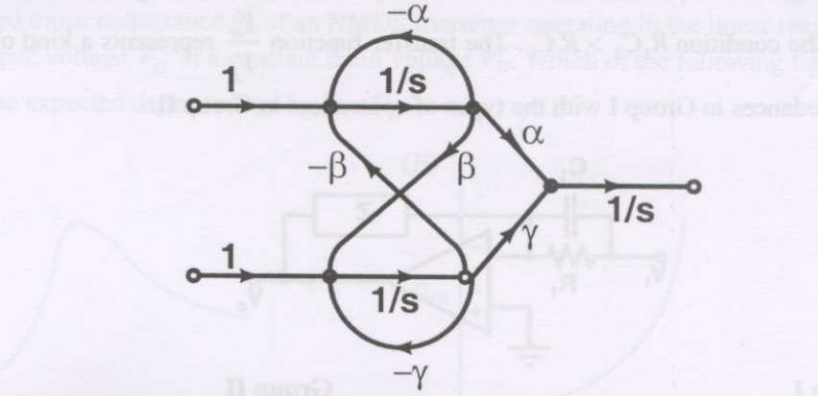
\includegraphics[width=0.5\columnwidth]{figs/q40.png}
\caption{Graph}
\label{fig:q40}
\end{figure}


The set of equations that correspond to this signal flow graph is
 
\noindent \textbf{[GATE EE 2025]}
\begin{enumerate}
  \item $\dfrac{d}{dt}
    \myvec {
      x_1 \\ x_2 \\ x_3
    }
    =
    \myvec {
      \beta & -\gamma & 0 \\
      \gamma & \alpha & 0 \\
      -\alpha & -\beta & 0
    }
    \myvec {
      x_1 \\ x_2 \\ x_3
    }
    +
    \myvec {
      1 & 0 \\
      0 & 1 \\
      0 & 0
    }
    \myvec {
      u_1 \\ u_2
    }
   $
  \item $\dfrac{d}{dt}
    \myvec {
      x_1 \\ x_2 \\ x_3
    }
    =
    \myvec {
      0 & \alpha & -\gamma \\
      -\gamma & 0 & \beta \\
      \alpha & \beta & 0
    }
    \myvec {
      x_1 \\ x_2 \\ x_3
    }
    +
    \myvec {
      1 & 0 \\
      0 & 1 \\
      0 & 0
    }
    \myvec {
      u_1 \\ u_2
    }
   $
  \item $\dfrac{d}{dt}
    \myvec {
      x_1 \\ x_2 \\ x_3
    }
    =
    \myvec {
      -\gamma & 0 & \beta \\
      \alpha & \gamma & 0 \\
      -\beta & 0 & -\alpha
    }
    \myvec {
      x_1 \\ x_2 \\ x_3
    }
    +
    \myvec {
      1 & 0 \\
      0 & 1 \\
      0 & 0
    }
    \myvec {
      u_1 \\ u_2
    }
   $
  \item $\dfrac{d}{dt}
    \myvec {
      x_1 \\ x_2 \\ x_3
    }
    =
    \myvec {
      -\gamma & 0 & \beta \\
      0 & \alpha & 0 \\
      -\beta & 0 & -\alpha
    }
    \myvec {
      x_1 \\ x_2 \\ x_3
    }
    +
    \myvec {
      1 & 0 \\
      0 & 1 \\
      0 & 0
    }
    \myvec {
      u_1 \\ u_2
    }
   $
\end{enumerate}

\item The number of open right half plane poles of $G(s) = \dfrac{10}{s^3 + 2s^4 + 3s^3 + 6s^2 + 5s + 3}$ is
 
\noindent \textbf{[GATE EE 2025]}
\begin{multicols}{4}
\begin{enumerate}
  \item 0
  \item 1
  \item 2
  \item 3
\end{enumerate}
\end{multicols}

\item The magnitude of frequency response of an underdamped second order system is 5 at 0 rad/sec and peaks to $\dfrac{10}{\sqrt{3}}$ at $5 \sqrt{2}$ rad/sec. The transfer function of the system is
 
\noindent \textbf{[GATE EE 2025]}
\begin{multicols}{4}
\begin{enumerate}
  \item $\dfrac{500}{s^2 + 10s + 100}$
  \item $\dfrac{375}{s^2 + 5s + 75}$
  \item $\dfrac{720}{s^2 + 12s + 144}$
  \item $\dfrac{1125}{s^2 + 25s + 225}$
\end{enumerate}
\end{multicols}

\item
Group I gives two possible choices for the impedance $Z$ in the diagram. The circuit elements in $Z$ satisfy the condition $R_2C_2 > R_1C_1$. The transfer function $\frac{V_o}{V_i}$ represents a kind of controller. Match the impedances in Group I with the types of controllers in Group II.
\begin{figure}[H]\centering
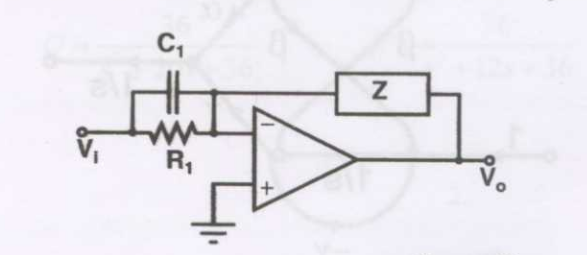
\includegraphics[width=0.8\columnwidth]{figs/q43a.png}
\caption{Circuit}
\label{fig:q43a}
\end{figure}
\textbf{Group I:}

\begin{figure}[H]\centering
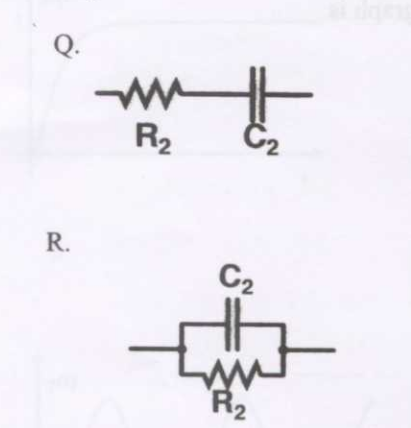
\includegraphics[width=0.4\columnwidth]{figs/q43b.png}
\caption{Group I}
\label{fig:q43b}
\end{figure}

\textbf{Group II:}

1. PID controller\hspace{1em}
2. Lead compensator\hspace{1em}
3. Lag compensator
 
\noindent \textbf{[GATE EE 2025]}
\begin{multicols}{4}
\begin{enumerate}
  \item Q-1, R-2
  \item Q-1, R-3
  \item Q-2, R-3
  \item Q-3, R-2
\end{enumerate}
\end{multicols}

\item For the circuit shown in the following figure, transistors M1 and M2 are identical NMOS transistors. Assume that M2 is in saturation and the output is unloaded.
\begin{figure}[H]\centering
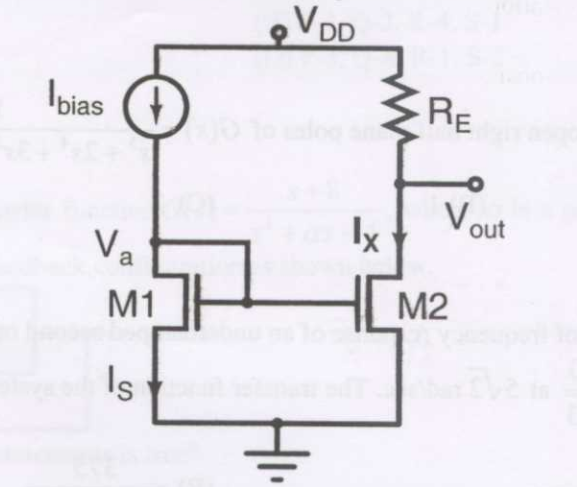
\includegraphics[width=0.5\columnwidth]{figs/q44.png}
\caption{Circuit}
\label{fig:q44}
\end{figure}

The current $I_X$ is related to $I_{bias}$ as
 
\noindent \textbf{[GATE EE 2025]}
\begin{multicols}{2}
\begin{enumerate}
  \item $I_X = I_{bias} + I_S$
  \item $I_X = I_{bias}$
  \item $I_X = I_{bias} - I_S$
  \item $I_X = I_{bias}\left( \dfrac{V_{DD} - V_{out}}{R_E} \right)$
\end{enumerate}
\end{multicols}

\item The measured transconductance $g_m$ of an NMOS transistor operating in the linear region is plotted against the gate voltage $V_G$ at a constant drain voltage $V_D$. Which of the following figures represents the expected dependence of $g_m$ on $V_G$?
 
\noindent \textbf{[GATE EE 2025]}
\begin{figure}[H]\centering
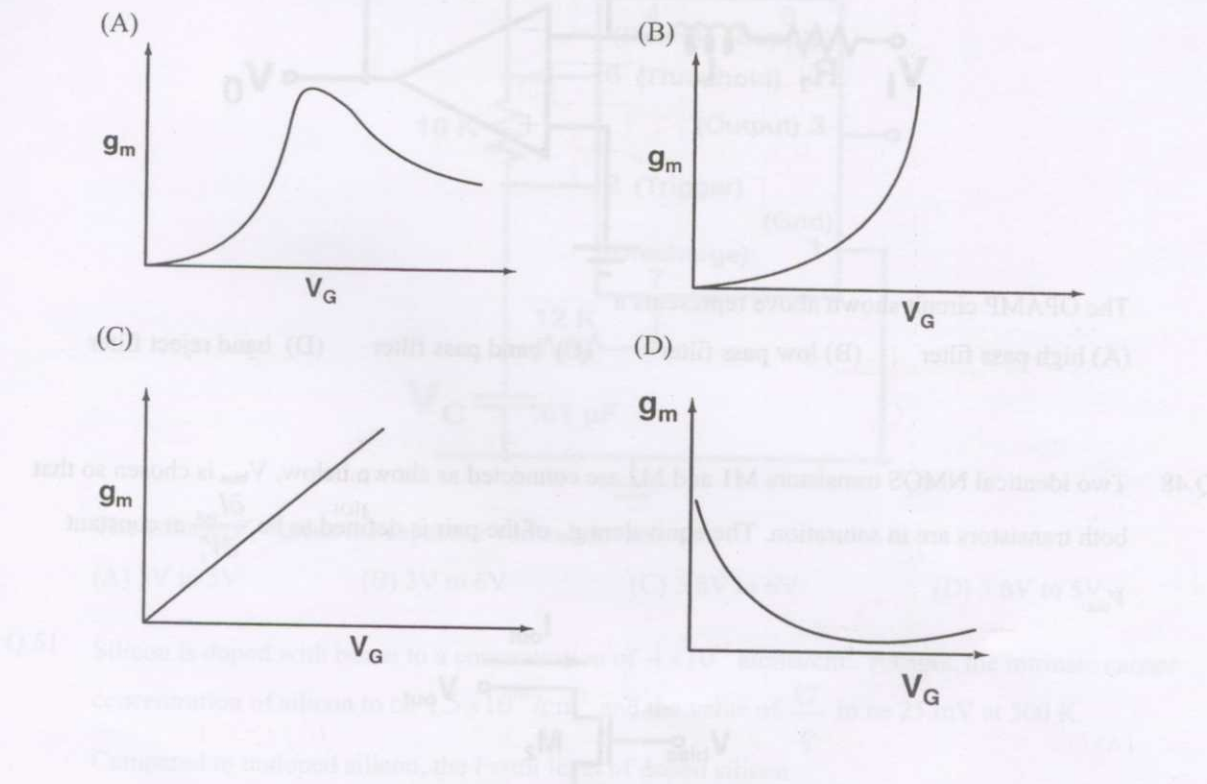
\includegraphics[width=0.95\columnwidth]{figs/q45.png}
\caption{Options}
\label{fig:q45}
\end{figure}

\item Consider the following circuit using an ideal OPAMP. The I-V characteristics of the diode is described by the relation $I = I_0 \left( e^{V/V_T} - 1 \right)$ where $V_T = 25\text{ mV}$, $I_0 = 1\,\mu A$ and $V$ is the voltage across the diode (taken as positive for forward bias).

\begin{figure}[H]\centering
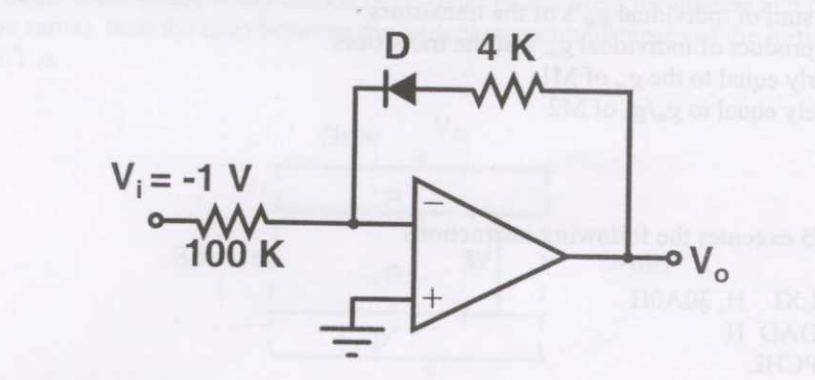
\includegraphics[width=0.5\columnwidth]{figs/q46.png}
\caption{Circuit}
\label{fig:q46}
\end{figure}

For an input voltage $V_i = -1$ V, the output voltage $V_o$ is
 
\noindent \textbf{[GATE EE 2025]}
\begin{multicols}{4}
\begin{enumerate}
  \item 0 V
  \item 0.1 V
  \item 0.7 V
  \item 1.1 V
\end{enumerate}
\end{multicols}

\item The OPAMP circuit shown above represents a
 
\noindent \textbf{[GATE EE 2025]}
\begin{figure}[H]\centering
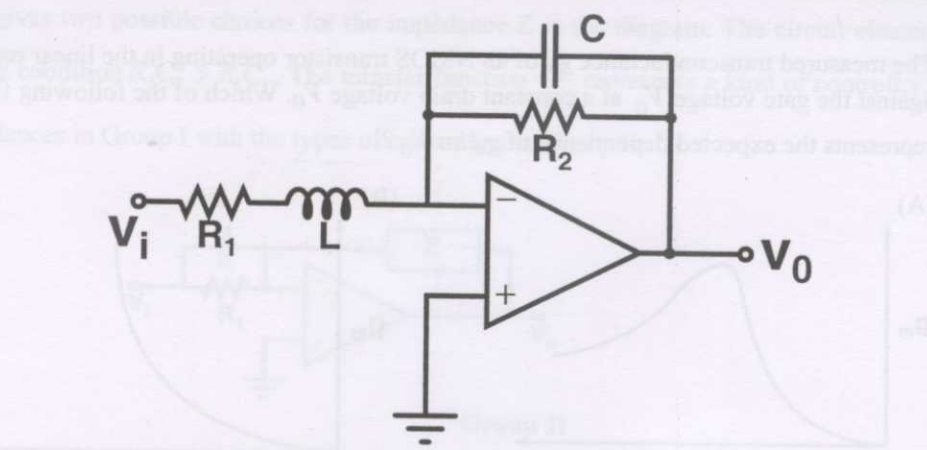
\includegraphics[width=0.5\columnwidth]{figs/q47.png}
\caption{Circuit}
\label{fig:q47}
\end{figure}

\begin{multicols}{2}
\begin{enumerate}
  \item high pass filter
  \item low pass filter
  \item band pass filter
  \item band reject filter
\end{enumerate}
\end{multicols}

\item Two identical NMOS transistors $M_1$ and $M_2$ are connected as shown below. $V_{bias}$ is chosen so that both transistors are in saturation. The equivalent $g_m$ of the pair is defined to be $\left. \frac{\partial I_{out}}{\partial V_i} \right|_{const\, V_{out}}$.

\begin{figure}[H]\centering
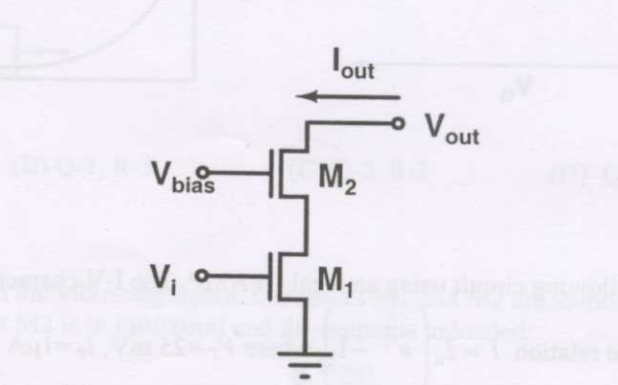
\includegraphics[width=0.5\columnwidth]{figs/q48.png}
\caption{Circuit}
\label{fig:q48}
\end{figure}

The equivalent $g_m$ of the pair is
 
\noindent \textbf{[GATE EE 2025]}
\begin{enumerate}
  \item the sum of individual $g_m$'s of the transistors
  \item the product of individual $g_m$'s of the transistors
  \item nearly equal to the $g_m$ of $M_1$
  \item nearly equal to $g_m/g_{0}$ of $M_2$
\end{enumerate}

\item An 8085 executes the following instructions:

LXI H, 30A0H

DAD H

PCHL

All addresses and constants are in Hex. Let PC be the contents of the program counter and HL be the contents of the HL register pair just after executing PCHL.

Which of the following statements is correct?
 
\noindent \textbf{[GATE EE 2025]}
\begin{multicols}{2}
\begin{enumerate}
  \item PC = 2715H,\quad HL = 30A0H
  \item PC = 30A0H,\quad HL = 2715H
  \item PC = 6140H,\quad HL = 6140H
  \item PC = 6140H,\quad HL = 2715H
\end{enumerate}
\end{multicols}

\item An astable multivibrator circuit using IC 555 timer is shown below. Assume that the circuit is oscillating steadily.

\begin{figure}[H]\centering
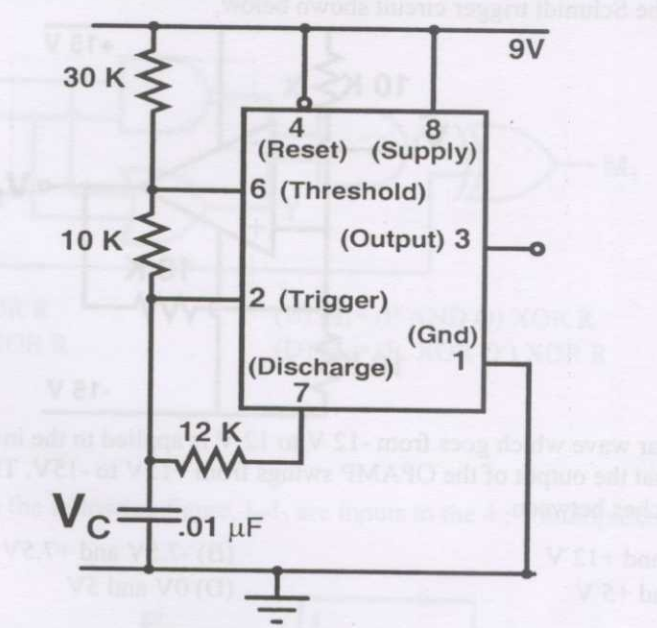
\includegraphics[width=0.7\columnwidth]{figs/q50.png}
\caption{Circuit}
\label{fig:q50}
\end{figure}

The voltage $V_C$ across the capacitor varies between
 
\noindent \textbf{[GATE EE 2025]}
\begin{multicols}{4}
\begin{enumerate}
    \item $3$ V to $5$ V
    \item $3$ V to $6$ V
    \item $3.6$ V to $6$ V
    \item $3.6$ V to $5$ V
\end{enumerate}
\end{multicols}

\item Silicon is doped with boron to a concentration of $4 \times 10^{17}$ atoms/cm$^3$. Assume the intrinsic carrier concentration of silicon to be $1.5\times10^{10}$/cm$^3$ and the value of $kT/q$ to be 25 mV at 300 K. Compared to undoped silicon, the Fermi level of doped silicon
 
\noindent \textbf{[GATE EE 2025]}
\begin{multicols}{2}
\begin{enumerate}
    \item goes down by $0.13$ eV
    \item goes up by $0.13$ eV
    \item goes down by $0.427$ eV
    \item goes up by $0.427$ eV
\end{enumerate}
\end{multicols}

\item The cross section of a JFET is shown in the following figure. Let $V_G$ be $-2$V and let $V_p$ be the initial pinch-off voltage. If the width $W$ is doubled (other geometrical parameters and doping levels remaining the same), then the ratio between the mutual transconductances of the initial and the modified JFET is

\begin{figure}[H]\centering
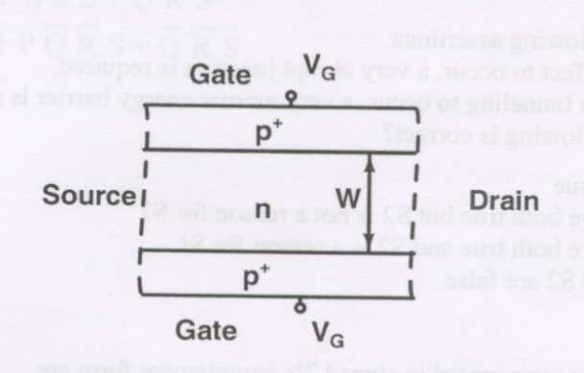
\includegraphics[width=0.5\columnwidth]{figs/q52.png}
\caption{Diagram}
\label{fig:q52}
\end{figure}
 
\noindent \textbf{[GATE EE 2025]}
\begin{multicols}{2}
\begin{enumerate}
    \item 4
    \item $\dfrac{1 - \sqrt{2/V_p'}}{1 - \sqrt{1/(2V_p')}}$
    \item $\dfrac{1 - \sqrt{2/V_p}}{1 - \sqrt{1/(2V_p)}}$
    \item $\dfrac{1 - (2/\sqrt{V_p})}{1 - (1/(2\sqrt{V_p}))}$
\end{enumerate}
\end{multicols}

\item Consider the Schmidt trigger circuit shown below.

\begin{figure}[H]\centering
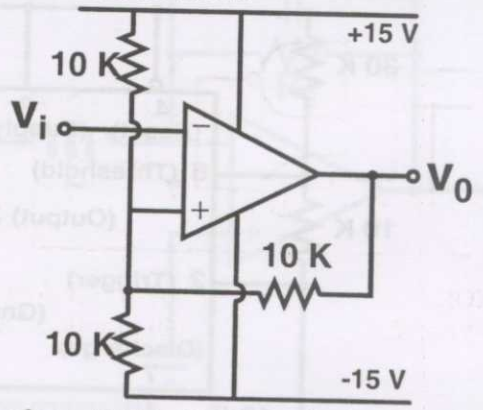
\includegraphics[width=0.5\columnwidth]{figs/q53.png}
\caption{Circuit}
\label{fig:q53}
\end{figure}

A triangular wave which goes from $-12$ V to $12$ V is applied to the inverting input of the OPAMP. Assume that the output of the OPAMP swings from $+15$ V to $-15$ V. The voltage at the non-inverting input switches between
 
\noindent \textbf{[GATE EE 2025]}
\begin{multicols}{2}
\begin{enumerate}
    \item $-12$ V and $+12$ V
    \item $-7.5$ V and $+7.5$ V
    \item $-5$ V and $+5$ V
    \item $0$ V and $5$ V
\end{enumerate}
\end{multicols}

\item The logic function implemented by the following circuit at the terminal OUT is
\begin{figure}[H]\centering
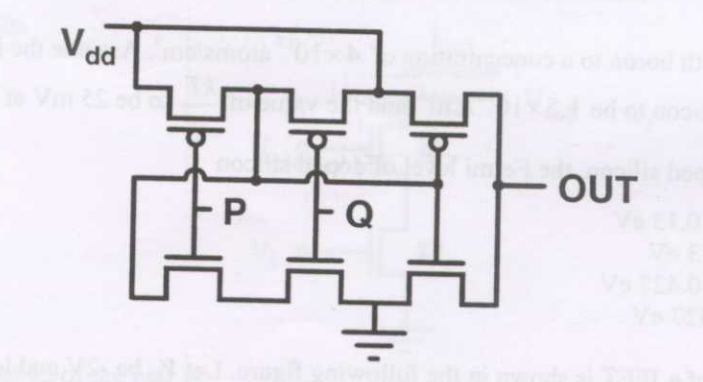
\includegraphics[width=0.6\columnwidth]{figs/q54.png}
\caption{Circuit}
\label{fig:q54}
\end{figure}
 
\noindent \textbf{[GATE EE 2025]}
\begin{multicols}{4}
\begin{enumerate}
    \item $P$ NOR $Q$
    \item $P$ NAND $Q$
    \item $P$ OR $Q$
    \item $P$ AND $Q$
\end{enumerate}
\end{multicols}

\item Consider the following assertions. \\
S1: For Zener effect to occur, a very abrupt junction is required. \\
S2: For quantum tunneling to occur, a very narrow energy barrier is required.

Which of the following is correct?
 
\noindent \textbf{[GATE EE 2025]}
\begin{enumerate}
    \item Only S2 is true
    \item S1 and S2 are both true but S2 is not a reason for S1
    \item S1 and S2 are both true and S2 is a reason for S1
    \item Both S1 and S2 are false
\end{enumerate}

\item The two numbers represented in signed $2$'s complement form are \\
$P=11101101$ and $Q=11100110$. If $Q$ is subtracted from $P$, the value obtained in signed $2$'s complement form is
 
\noindent \textbf{[GATE EE 2025]}
\begin{multicols}{4}
\begin{enumerate}
    \item 100000111
    \item 00000111
    \item 11111001
    \item 111111001
\end{enumerate}
\end{multicols}

\item Which of the following Boolean Expressions correctly represents the relation between $P, Q, R$ and $M_1$?
\begin{figure}[H]\centering
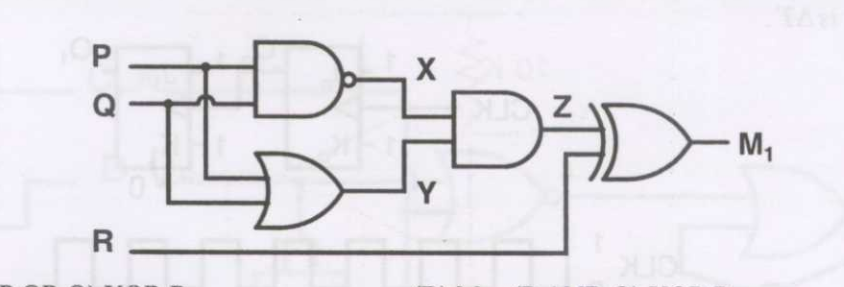
\includegraphics[width=0.6\columnwidth]{figs/q57.png}
\caption{Circuit}
\label{fig:q57}
\end{figure}
 
\noindent \textbf{[GATE EE 2025]}
\begin{multicols}{2}
\begin{enumerate}
  \item $M_1 = (P \text{ OR } Q) \text{ XOR } R$
  \item $M_1 = (P \text{ AND } Q) \text{ XOR } R$
  \item $M_1 = (P \text{ NOR } Q) \text{ XOR } R$
  \item $M_1 = (P \text{ XOR } Q) \text{ XOR } R$
\end{enumerate}
\end{multicols}

\item For the circuit shown in the following figure, $I_0$–$I_3$ are inputs to the 4:1 multiplexer. $R$ (MSB) and $S$ are control bits. The output $Z$ can be represented by
\begin{figure}[H]\centering
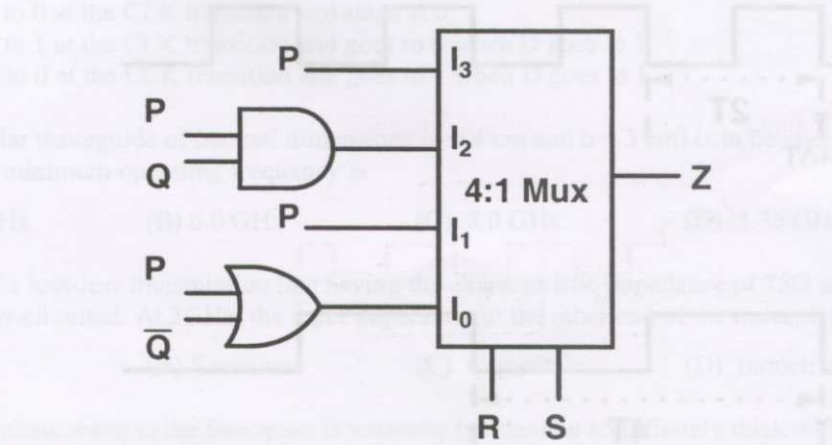
\includegraphics[width=0.6\columnwidth]{figs/q58.png}
\caption{Circuit}
\label{fig:q58}
\end{figure}
 
\noindent \textbf{[GATE EE 2025]}
\begin{multicols}{2}
\begin{enumerate}
  \item $PQ + P\overline{Q}S + \overline{Q}\, \overline{R}S$
  \item $P\overline{Q} + PQR + \overline{P}\, \overline{Q}S$
  \item $P\overline{Q}R + \overline{P}QR + P Q R S + \overline{Q}\overline{R}S$
  \item $P Q \overline{R} + P Q R \overline{S} + P\overline{Q}RS + \overline{Q}R\overline{S}$
\end{enumerate}
\end{multicols}

\item For each of the positive edge-triggered J-K flip flop used in the following figure, the propagation delay is $\Delta T$.

\begin{figure}[H]\centering
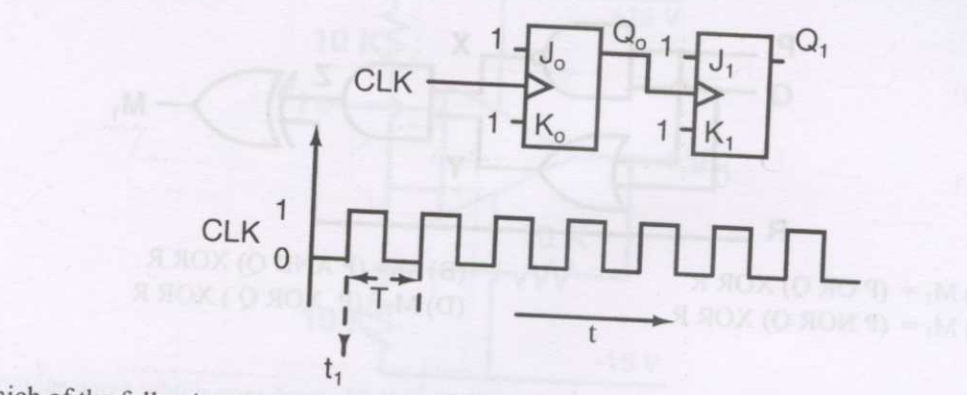
\includegraphics[width=0.6\columnwidth]{figs/q59a.png}
\caption{Diagram}
\label{fig:q59a}
\end{figure}

Which of the following waveforms correctly represents the output at $Q_1$?
 
\noindent \textbf{[GATE EE 2025]}
\begin{figure}[H]\centering
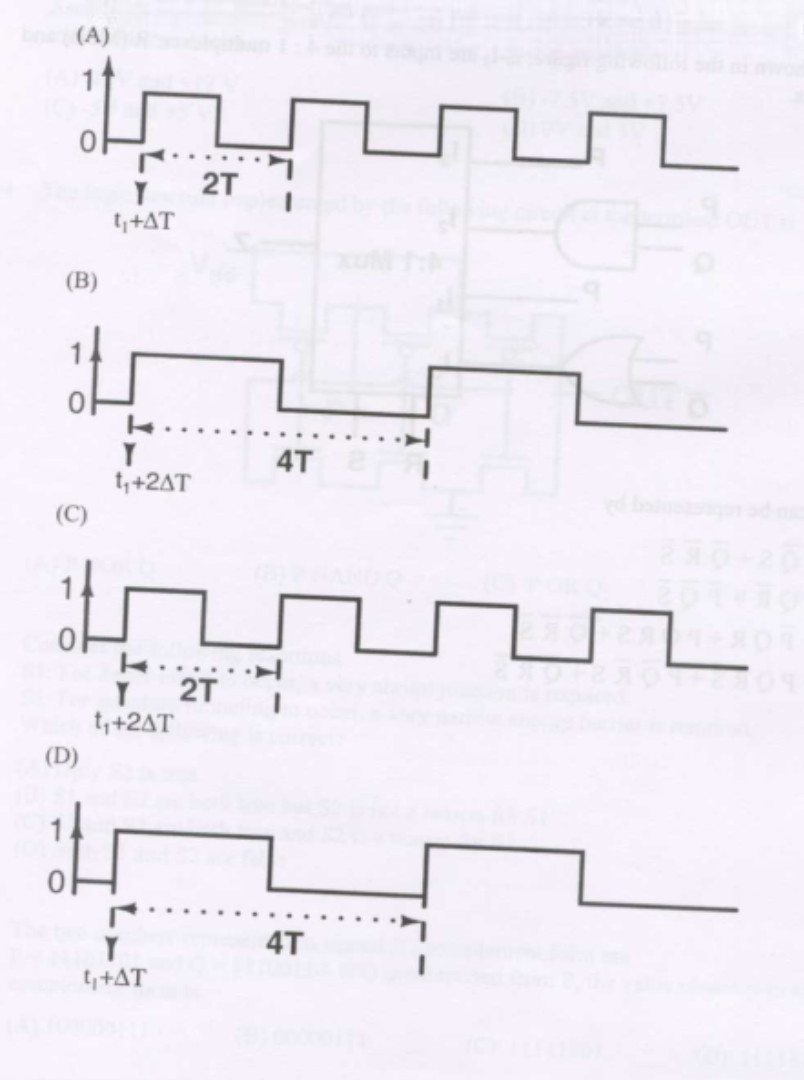
\includegraphics[width=0.7\columnwidth]{figs/q59b.png}
\caption{Options}
\label{fig:q59b}
\end{figure}

\item For the circuit shown in the figure, $D$ has a transition from 0 to 1 after CLK changes from 1 to 0. Assume gate delays to be negligible.

\begin{figure}[H]\centering
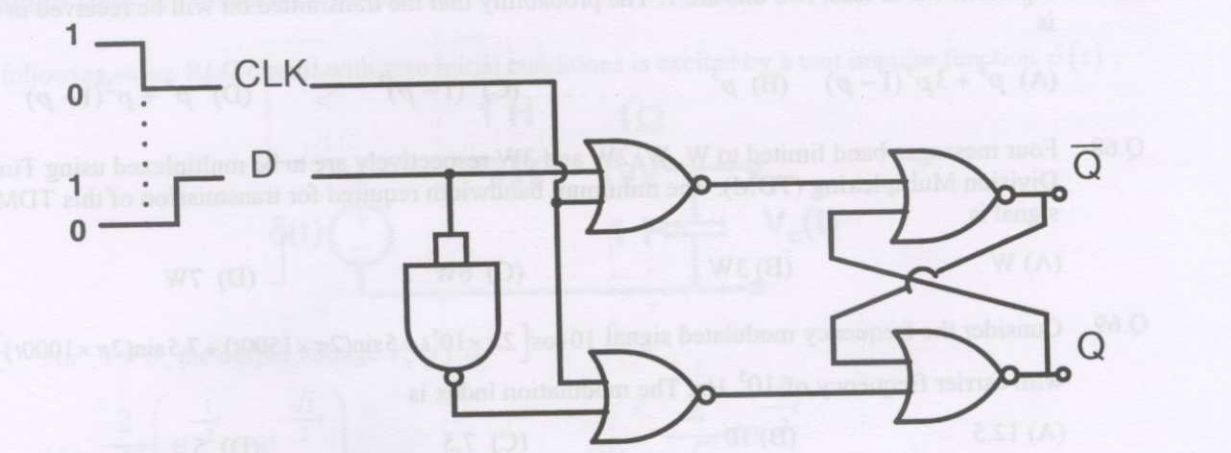
\includegraphics[width=0.6\columnwidth]{figs/q60.png}
\caption{Circuit}
\label{fig:q60}
\end{figure}

Which of the following statements is true?
 
\noindent \textbf{[GATE EE 2025]}
\begin{enumerate}
  \item $Q$ goes to 1 at the CLK transition and stays at 1.
  \item $Q$ goes to 0 at the CLK transition and stays at 0.
  \item $Q$ goes to 1 at the CLK transition and goes to 0 when $D$ goes to 1.
  \item $Q$ goes to 0 at the CLK transition and goes to 1 when $D$ goes to 1.
\end{enumerate}

\item A rectangular waveguide of internal dimensions ($a=4$ cm and $b=3$ cm) is to be operated in $\mathrm{TE}_{11}$ mode. The minimum operating frequency is
 
\noindent \textbf{[GATE EE 2025]}
\begin{multicols}{4}
\begin{enumerate}
  \item 6.25 GHz
  \item 6.0 GHz
  \item 5.0 GHz
  \item 3.75 GHz
\end{enumerate}
\end{multicols}

\item One end of a loss-less transmission line having the characteristic impedance of $75\;\ohm$ and length of 1 cm is short-circuited. At 3 GHz, the input impedance at the other end of the transmission line is
 
\noindent \textbf{[GATE EE 2025]}
\begin{multicols}{4}
\begin{enumerate}
  \item 0
  \item Resistive
  \item Capacitive
  \item Inductive
\end{enumerate}
\end{multicols}

\item A uniform plane wave in free space is normally incident on an infinitely thick dielectric slab (dielectric constant $\epsilon_r = 9$). The magnitude of the reflection coefficient is
 
\noindent \textbf{[GATE EE 2025]}
\begin{multicols}{4}
\begin{enumerate}
  \item 0
  \item 0.3
  \item 0.5
  \item 0.8
\end{enumerate}
\end{multicols}

\item In the design of a single mode step index optical fiber close to upper cut-off, the single-mode operation is NOT preserved if
 
\noindent \textbf{[GATE EE 2025]}
\begin{enumerate}
  \item radius as well as operating wavelength are halved
  \item radius as well as operating wavelength are doubled
  \item radius is halved and operating wavelength is doubled
  \item radius is doubled and operating wavelength is halved
\end{enumerate}

\item At 20 GHz, the gain of a parabolic dish antenna of 1 meter diameter and 70\% efficiency is
 
\noindent \textbf{[GATE EE 2025]}
\begin{multicols}{4}
\begin{enumerate}
  \item 15 dB
  \item 25 dB
  \item 35 dB
  \item 45 dB
\end{enumerate}
\end{multicols}

\item Noise with double-sided power spectral density $K$ over all frequencies is passed through a RC low pass filter with 3 dB cut-off frequency of $f_c$. The noise power at the filter output is
 
\noindent \textbf{[GATE EE 2025]}
\begin{multicols}{4}
\begin{enumerate}
  \item $K$
  \item $K f_c$
  \item $K \pi f_c$
  \item $\infty$
\end{enumerate}
\end{multicols}

\item Consider a Binary Symmetric Channel (BSC) with probability of error being $p$. To transmit a bit, say 1, we transmit a sequence of three 1s. The receiver will interpret the received sequence to represent 1 if at least two bits are 1. The probability that the transmitted bit will be received in error is
 
\noindent \textbf{[GATE EE 2025]}
\begin{multicols}{2}
\begin{enumerate}
  \item $p^3 + 3p^2(1-p)$
  \item $p^3$
  \item $(1-p)^3$
  \item $p^3 + p^2(1-p)$
\end{enumerate}
\end{multicols}

\item Four messages band limited to $W, W, 2W$ and $3W$ respectively are to be multiplexed using Time Division Multiplexing (TDM). The minimum bandwidth required for transmission of this TDM signal is
 
\noindent \textbf{[GATE EE 2025]}
\begin{multicols}{4}
\begin{enumerate}
  \item $W$
  \item $3W$
  \item $6W$
  \item $7W$
\end{enumerate}
\end{multicols}

\item Consider the frequency modulated signal $10\cos[2\pi \times 10^5 t + 5\sin(2\pi \times 1500 t) + 7.5\sin(2\pi \times 1000 t)]$ with carrier frequency of $10^5$ Hz. The modulation index is
 
\noindent \textbf{[GATE EE 2025]}
\begin{multicols}{4}
\begin{enumerate}
  \item 12.5
  \item 10
  \item 7.5
  \item 5
\end{enumerate}
\end{multicols}

\item The signal $\cos \ohm_1 t + 0.5 \cos \ohm_f t \sin \ohm_t t$ is
 
\noindent \textbf{[GATE EE 2025]}
\begin{multicols}{2}
\begin{enumerate}
  \item FM only
  \item AM only
  \item both AM and FM
  \item neither AM nor FM
\end{enumerate}
\end{multicols}

\end{enumerate}


 \large \textbf {Common Data Questions}
 \large \textbf {Common Data for Questions 71, 72, 73}

 
A speech signal, band limited to 4 kHz and peak voltage varying between +5V and -5V, is sampled at the Nyquist rate. Each sample is quantized and represented by 8 bits.

\begin{enumerate}[leftmargin=*, label=\textbf{Q.\arabic*:}]
\setcounter{enumi}{70}

\item If the bits 0 and 1 are transmitted using bipolar pulses, the minimum bandwidth required for distortion free transmission is
 
\noindent \textbf{[GATE EE 2025]}
\begin{multicols}{4}
\begin{enumerate}
  \item 64 kHz
  \item 32 kHz
  \item 8 kHz
  \item 4 kHz
\end{enumerate}
\end{multicols}

\item Assuming the signal to be uniformly distributed between its peak to peak value, the signal to noise ratio at the quantizer output is
 
\noindent \textbf{[GATE EE 2025]}
\begin{multicols}{4}
\begin{enumerate}
  \item 16 dB
  \item 32 dB
  \item 48 dB
  \item 64 dB
\end{enumerate}
\end{multicols}

\item The number of quantization levels required to reduce the quantization noise by a factor of 4 would be
 
\noindent \textbf{[GATE EE 2025]}
\begin{multicols}{4}
\begin{enumerate}
  \item 1024
  \item 512
  \item 256
  \item 64
\end{enumerate}
\end{multicols}

\end{enumerate}


 \large \textbf {Common Data for Questions 74,75}


\begin{enumerate}
\item The following series RLC circuit with zero initial conditions is excited by a unit impulse function $\delta(t)$.
\end{enumerate}
 
\begin{figure}[H]\centering
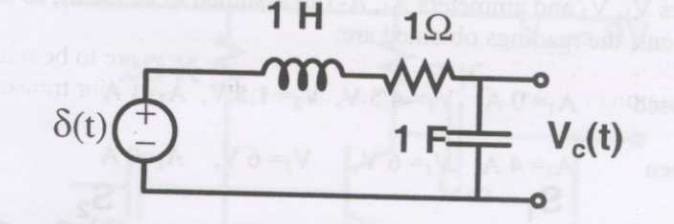
\includegraphics[width=0.6\columnwidth]{figs/q7475.png}
\caption{Circuit}
\label{fig:q7475}
\end{figure}

\begin{enumerate}[leftmargin=*, label=\textbf{Q.\arabic*:}]
\setcounter{enumi}{73}

\item For $t>0$, the output voltage $V_c(t)$ is
 
\noindent \textbf{[GATE EE 2025]}
\begin{multicols}{2}
\begin{enumerate}
  \item $\dfrac{2}{\sqrt{3}}\left(e^{-\frac{1}{2}t} - e^{-\frac{\sqrt{3}}{2}t}\right)$
  \item $\dfrac{2}{\sqrt{3}} t e^{-\frac{1}{2} t}$
  \item $\dfrac{2}{\sqrt{3}} e^{-\frac{1}{2} t} \cos\left( \dfrac{\sqrt{3}}{2} t \right)$
  \item $\dfrac{2}{\sqrt{3}} e^{-\frac{1}{2} t} \sin\left( \dfrac{\sqrt{3}}{2} t \right)$
\end{enumerate}
\end{multicols}

\item For $t>0$, the voltage across the resistor is
 
\noindent \textbf{[GATE EE 2025]}
\begin{multicols}{2}
\begin{enumerate}
  \item $\dfrac{1}{\sqrt{3}} \left( e^{-\frac{\sqrt{3}}{2} t} - e^{-\frac{1}{2} t} \right)$
  \item $e^{-\frac{1}{2} t} \left[ \cos \left( \dfrac{\sqrt{3}}{2} t \right) - \dfrac{1}{\sqrt{3}} \sin \left( \dfrac{\sqrt{3}}{2} t \right) \right]$
  \item $\dfrac{2}{\sqrt{3}} e^{-\frac{1}{2} t} \sin \left( \dfrac{\sqrt{3}}{2} t \right)$
  \item $\dfrac{2}{\sqrt{3}} e^{-\frac{1}{2} t} \cos \left( \dfrac{\sqrt{3}}{2} t \right)$
\end{enumerate}
\end{multicols}

\end{enumerate}


 \large \textbf {Linked Answer Questions: Q.76 to Q.85 carry two marks each}
 \large \textbf {Statement for Linked Answer Questions 76 and 77: }

\begin{enumerate}
\item A two-port network shown below is excited by external dc sources. The voltages and the currents are measured with voltmeters V1, V2 and ammeters A1, A2 (all assumed to be ideal), as indicated. Under following switch conditions, the readings obtained are: \\
(i) $S_1$ open, $S_2$ closed: $A_1=0$ A, $V_1=4.5$ V, $V_2=1.5$ V, $A_2=1$ A \\
(ii) $S_1$ closed, $S_2$ open: $A_1=4$ A, $V_1=6$ V, $V_2=6$ V, $A_2=0$ A
\end{enumerate}
\begin{figure}[H]\centering
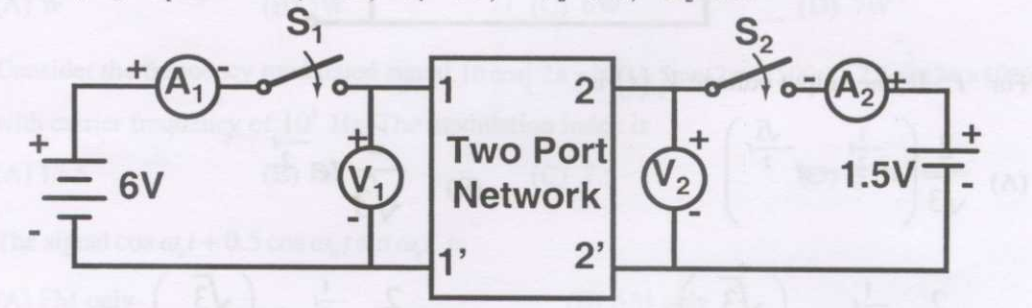
\includegraphics[width=0.6\columnwidth]{figs/q7677.png}
\caption{Circuit}
\label{fig:q7677}
\end{figure}

\begin{enumerate}[leftmargin=*, label=\textbf{Q.\arabic*:}]
\setcounter{enumi}{75}

\item The $z$-parameter matrix for this network is
 
\noindent \textbf{[GATE EE 2025]}
\begin{multicols}{4}
\begin{enumerate}
  \item $\myvec { 1.5 & 1.5 \\ 4.5 & 1.5 }$
  \item $\myvec { 1.5 & 4.5 \\ 1.5 & 4.5 }$
  \item $\myvec { 1.5 & 1.5 \\ 1.5 & 1.5 }$
  \item $\myvec { 4.5 & 1.5 \\ 1.5 & 4.5 }$
\end{enumerate}
\end{multicols}

\item The $h$-parameter matrix for this network is
 
\noindent \textbf{[GATE EE 2025]}
\begin{multicols}{4}
\begin{enumerate}
  \item $\myvec { -3 & 0.8 \\ -1 & 0.67 }$
  \item $\myvec { 3 & 0.67 \\ 1 & 0.67 }$
  \item $\myvec { 1 & 0.67 \\ 3 & 0.67 }$
  \item $\myvec { -3 & -0.67 \\ 1 & 0.67 }$
\end{enumerate}
\end{multicols}

\end{enumerate}


 \large \textbf {Linked Answer Questions: Q.76 to Q.85 carry two marks each}
 \large \textbf {Statement for Linked Answer Questions 78 and 79: }

 \begin{enumerate}
\item In the following network, the switch is closed at $t=0$ and the sampling starts from $t=0$. The sampling frequency is $10$ Hz.
\end{enumerate}
\begin{figure}[H]\centering
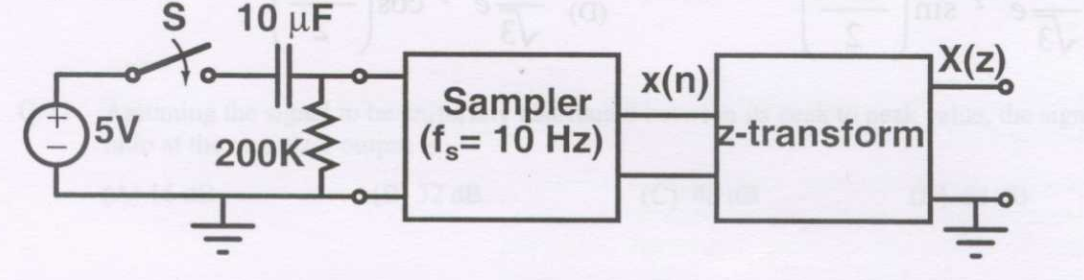
\includegraphics[width=0.6\columnwidth]{figs/q7879.png}
\caption{Circuit}
\label{fig:q7879}
\end{figure}

\begin{enumerate}[leftmargin=*, label=\textbf{Q.\arabic*:}]
\setcounter{enumi}{77}

\item The samples $x(n)$ ($n=0,1,2,\ldots$) are given by
 
\noindent \textbf{[GATE EE 2025]}
\begin{multicols}{4}
\begin{enumerate}
  \item $5 \left( 1 - e^{-0.05 n} \right)$
  \item $5 e^{-0.05 n}$
  \item $5 \left( 1 - e^{-5 n} \right)$
  \item $5 e^{-5 n}$
\end{enumerate}
\end{multicols}

\item The expression and the region of convergence of the $z$-transform of the sampled signal are
 
\noindent \textbf{[GATE EE 2025]}
\begin{multicols}{2}
\begin{enumerate}
  \item $\dfrac{5z}{z-e^{5}};~ |z|<e^{5}$
  \item $\dfrac{5z}{z-e^{-0.05}};~ |z|<e^{-0.05}$
  \item $\dfrac{5z}{z-e^{-0.05}};~ |z|>e^{-0.05}$
  \item $\dfrac{5z}{z-e^{5}};~ |z|>e^{5}$
\end{enumerate}
\end{multicols}

\end{enumerate}


 \large \textbf {Linked Answer Questions: Q.76 to Q.85 carry two marks each}
 \large \textbf {Statement for Linked Answer Questions 80 and 81: }

\begin{enumerate}
\item In the following transistor circuit, $V_{BE}=0.7$ V, $r_e = 25\,\text{mV}/I_E$, and $\beta$ and all the capacitances are very large. Under following switch conditions, the readings obtained are:
\end{enumerate}
\begin{figure}[H]\centering
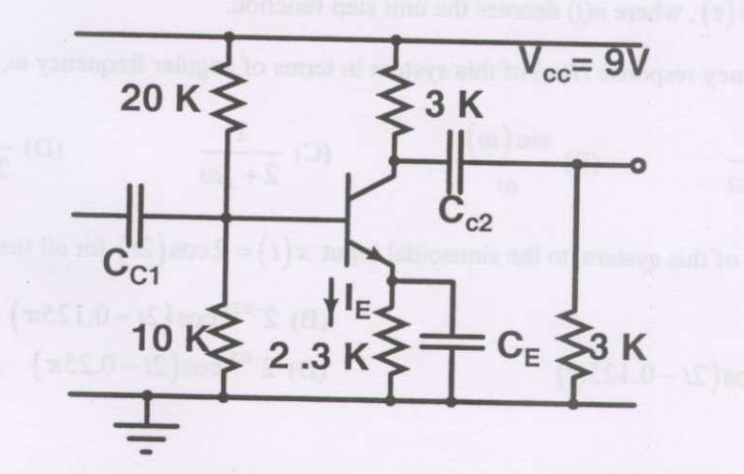
\includegraphics[width=0.6\columnwidth]{figs/q8081.png}
\caption{Circuit}
\label{fig:q8081}
\end{figure}

\begin{enumerate}[leftmargin=*, label=\textbf{Q.\arabic*:}]
\setcounter{enumi}{79}

\item The value of DC current $I_E$ is
 
\noindent \textbf{[GATE EE 2025]}
\begin{multicols}{4}
\begin{enumerate}
  \item 1 mA
  \item 2 mA
  \item 5 mA
  \item 10 mA
\end{enumerate}
\end{multicols}

\item The mid-band voltage gain of the amplifier is approximately
 
\noindent \textbf{[GATE EE 2025]}
\begin{multicols}{4}
\begin{enumerate}
  \item $-180$
  \item $-120$
  \item $-90$
  \item $-60$
\end{enumerate}
\end{multicols}

\end{enumerate}


 \large \textbf {Linked Answer Questions: Q.76 to Q.85 carry two marks each}
 \large \textbf {Statement for Linked Answer Questions 82 and 83: }

\begin{enumerate}
\item In the following circuit, the comparator output is logic “1” if $V_1 > V_2$ and is logic “0” otherwise. The D/A conversion is done as per the relation
\[
V_{DAC} = \sum_{n=0}^3 2^{-n} b_n
\]
Volts, where $b_3$ (MSB), $b_2$, $b_1$ and $b_0$ (LSB) are the counter outputs.
\end{enumerate}
\begin{figure}[H]\centering
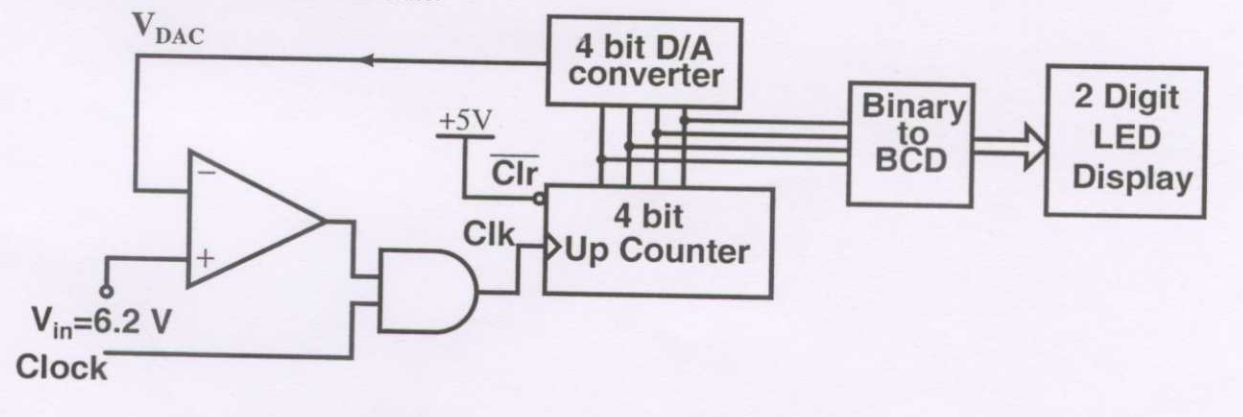
\includegraphics[width=0.6\columnwidth]{figs/q8283.png}
\caption{Circuit}
\label{fig:q8283}
\end{figure}

\begin{enumerate}[leftmargin=*, label=\textbf{Q.\arabic*:}]
\setcounter{enumi}{81}

\item The stable reading of the LED displays is
 
\noindent \textbf{[GATE EE 2025]}
\begin{multicols}{4}
\begin{enumerate}
  \item 06
  \item 07
  \item 12
  \item 13
\end{enumerate}
\end{multicols}

\item The magnitude of the error between $V_{DAC}$ and $V_{in}$ at steady state in volts is
 
\noindent \textbf{[GATE EE 2025]}
\begin{multicols}{4}
\begin{enumerate}
  \item 0.2
  \item 0.3
  \item 0.5
  \item 1.0
\end{enumerate}
\end{multicols}

\end{enumerate}


 \large \textbf {Linked Answer Questions: Q.76 to Q.85 carry two marks each}
 \large \textbf {Statement for Linked Answer Questions 84 and 85: }

\begin{enumerate}
\item The impulse response $h(t)$ of a linear time-invariant continuous time system is given by
$h(t) = \exp(-2 t) u(t)$, where $u(t)$ denotes the unit step function.
\end{enumerate}
\begin{enumerate}[leftmargin=*, label=\textbf{Q.\arabic*:}]
\setcounter{enumi}{83}

\item The frequency response $H(\ohm)$ of this system in terms of angular frequency $\ohm$, is given by $H(\ohm) = $
 
\noindent \textbf{[GATE EE 2025]}
\begin{multicols}{4}
\begin{enumerate}
  \item $\dfrac{1}{1 + j2\ohm}$
  \item $\dfrac{\sin \ohm}{\ohm}$
  \item $\dfrac{1}{2 + j\ohm}$
  \item $\dfrac{j\ohm}{2 + j\ohm}$
\end{enumerate}
\end{multicols}

\item The output of this system to the sinusoidal input $x(t) = 2 \cos (2t)$ for all time $t$ is
 
\noindent \textbf{[GATE EE 2025]}
\begin{multicols}{2}
\begin{enumerate}
  \item $0$
  \item $2^{-0.25} \cos (2t - 0.125\pi)$
  \item $2^{-0.5} \cos (2t - 0.125\pi)$
  \item $2^{-0.5} \cos (2t - 0.25\pi)$
\end{enumerate}
\end{multicols}

\end{enumerate}

\end{document}

